\documentclass[12pt, letterpaper]{article}
% --- Packages ---
\usepackage[utf8]{inputenc}
\usepackage{geometry}
\geometry{top=1in, bottom=1in, left=1in, right=1in}
\usepackage{graphicx}
\usepackage{xcolor}
\usepackage{mathptmx}
\usepackage{fancyhdr}
\usepackage{anyfontsize}
\usepackage{amsmath}
\usepackage{amssymb}
\usepackage{float}
\usepackage{caption}
\usepackage{subcaption}
\usepackage{listings}
\usepackage{mdframed}
\usepackage{titlesec}
\usepackage{booktabs}
\usepackage{needspace}
\usepackage{array}
\usepackage{hyperref}
% --- Color Definitions ---
\definecolor{cmured}{RGB}{196, 18, 48}
\definecolor{cmugrey}{RGB}{110, 110, 110}
\definecolor{codebg}{RGB}{245, 245, 245}
\definecolor{codeframe}{RGB}{196, 18, 48}
\definecolor{keywordcolor}{RGB}{0, 0, 180}
\definecolor{commentcolor}{RGB}{100, 100, 100}
\definecolor{stringcolor}{RGB}{150, 0, 0}
\hypersetup{colorlinks=true, linkcolor=cmured, urlcolor=cmured, citecolor=cmured}
% --- Header Settings ---
\setlength{\headheight}{25pt}
\pagestyle{fancy}
\fancyhf{}
\lhead{\small \scshape  Lab 3}
\rhead{\thepage}
\renewcommand{\headrulewidth}{1pt}
\renewcommand{\headrule}{\hbox to\headwidth{\color{cmured}\leaders\hrule height \headrulewidth\hfill}}
% --- Section Title Formatting ---
\titleformat{\section}
  {\large\bfseries\color{cmured}}
  {\thesection.}{0.5em}{}[\color{cmured}\titlerule]
\titleformat{\subsection}
  {\normalsize\bfseries\color{cmugrey}}
  {\thesubsection.}{0.5em}{}
% --- Caption Formatting (all captions centred and consistent) ---
\captionsetup{font=small, labelfont={bf,color=cmured}, labelsep=colon,
  justification=centering, singlelinecheck=false, skip=6pt}
\captionsetup[sub]{font=small, labelfont={bf,color=cmugrey},
  justification=centering, singlelinecheck=false, skip=4pt}
\captionsetup[lstlisting]{font=small, labelfont={bf,color=cmured}, labelsep=colon,
  justification=centering, singlelinecheck=false}
\renewcommand{\lstlistingname}{Listing}
% --- Images folder ---
\graphicspath{{images/}}
% --- Listings Style: shell / commands ---
\lstdefinestyle{shell}{
  backgroundcolor=\color{codebg},
  basicstyle=\ttfamily\small,
  breaklines=true,
  breakatwhitespace=false,
  frame=single,
  rulecolor=\color{codeframe},
  framesep=5pt,
  xleftmargin=10pt,
  xrightmargin=5pt,
  captionpos=b,
  showstringspaces=false,
  tabsize=2,
  keywordstyle=\color{keywordcolor}\bfseries,
  commentstyle=\color{commentcolor}\itshape,
  stringstyle=\color{stringcolor},
  numbers=none,
  columns=flexible,
}
\lstset{style=shell}
% --- Keep listings and headings from splitting across pages ---
\usepackage{etoolbox}
\BeforeBeginEnvironment{lstlisting}{\par\noindent\begin{minipage}{\linewidth}}
\AfterEndEnvironment{lstlisting}{\end{minipage}\par\medskip}
\pretocmd{\section}{\Needspace{10\baselineskip}}{}{}
\pretocmd{\subsection}{\Needspace{6\baselineskip}}{}{}
% ============================================================
\begin{document}
\emergencystretch=3em
% ============================================================
% -------------------------------------------------------
% COVER PAGE
% -------------------------------------------------------
\begin{titlepage}
  \thispagestyle{empty}
  \noindent
  {\small Course: Processing World Information} \hfill {\textbf{\today}}
  \vspace{3cm}
  \begin{flushleft}
    {\fontsize{55}{50}\selectfont \textbf{\textcolor{cmured}{Carnegie}}}\\[4mm]
    {\fontsize{55}{50}\selectfont \textbf{\textcolor{cmured}{Mellon}}}\\[4mm]
    {\fontsize{55}{50}\selectfont \textbf{\textcolor{cmured}{University}}}\\[2mm]
    {\fontsize{45}{50}\selectfont \textbf{\textcolor{cmugrey}{Africa}}}
  \end{flushleft}
  \vfill
  \begin{flushleft}
    \textbf{Name:} Martin Koome \\
    \vspace{0.2cm}
    \textbf{Course:} Processing World Information, Fall 2026
  \end{flushleft}
  \vspace{1.5cm}
  \begin{center}
    \large \textbf{Lab 3} \\[0.5cm]
    \large \textbf{Power Spectrum Analysis and Noise Removal}
  \end{center}
  \vspace{2cm}
\end{titlepage}

% -------------------------------------------------------
% SETUP
% -------------------------------------------------------
\section{Setup}

All results in this report were produced with the application built for this lab. It is a Tkinter program with two tabs. The Power Spectrum tab shows the spectrum of a block, the average spectrum, or a spectrogram. The Noise Filter tab applies one filter at a time to an audio or image file, shows before and after, and saves the result. The files are listed in \texttt{README.md}.

The processing used for every result is as follows.
\begin{itemize}
  \item \textbf{Transform.} The orthonormal real transform from class, computed with an FFT. For a block of $N$ samples, coefficient $k$ with $1 \le k < N/2$ is the cosine component at frequency $kF_s/N$ and coefficient $N-k$ is the sine component at the same frequency. The power at bin $k$ is $P_k = c_k^2 + c_{N-k}^2$. There are $N/2+1$ bins, each $F_s/N$ wide.
  \item \textbf{Blocks.} Non-overlapping blocks of $N$ samples. The last block is padded with zeros. No mean is removed.
  \item \textbf{Window.} Rectangular, Hamming or Hanning, applied to each block before the transform. Power is divided by $\sum w^2/N$, so levels can be compared between windows.
  \item \textbf{Display.} Power is shown in dB relative to the largest value in the view and clipped at a floor, which is stated in each figure. In the spectrograms blue is the floor and red is 0 dB. When several blocks are averaged, the linear power is averaged before conversion to dB.
  \item \textbf{Audio filters.} Median with threshold (a sample is replaced by the median of its neighbours only if it differs from it by more than the threshold, on a scale of $-1$ to $1$). Notch (band-reject) and lowpass, both Butterworth, order 4, applied forwards and backwards so they add no delay.
  \item \textbf{Image filters.} Median and Gaussian, applied to each colour channel separately.
  \item \textbf{Scoring.} I judged the audio by listening and by the spectrograms. As a check I also scored each result against the clean file supplied with the lab. For audio, $\mathrm{SNR} = 10\log_{10}\!\big(\mathrm{var}(x)/\mathrm{mean}((y-x)^2)\big)$ in dB, where $x$ is the clean signal and $y$ the signal being scored. For images I use PSNR with a peak value of 1. A higher number is better. These numbers are a guide and do not replace listening or looking.
\end{itemize}

% -------------------------------------------------------
% PART I
% -------------------------------------------------------
\section{Part I: Power Spectrum Analysis}

\subsection{Spectrogram of the C scale (step 3)}

Figure~\ref{fig:cscale2048} shows the spectrogram of \texttt{c\_scale.wav} ($F_s = 16$ kHz, 8 s). The frequency axis is limited to 0 to 1000 Hz, because all the notes are below 530 Hz. The scale has eight notes of one second each, at about 262, 293, 330, 350, 393, 440, 494 and 523 Hz (C4 to C5), so each note is easy to see as a horizontal line.

\begin{figure}[H]
  \centering
  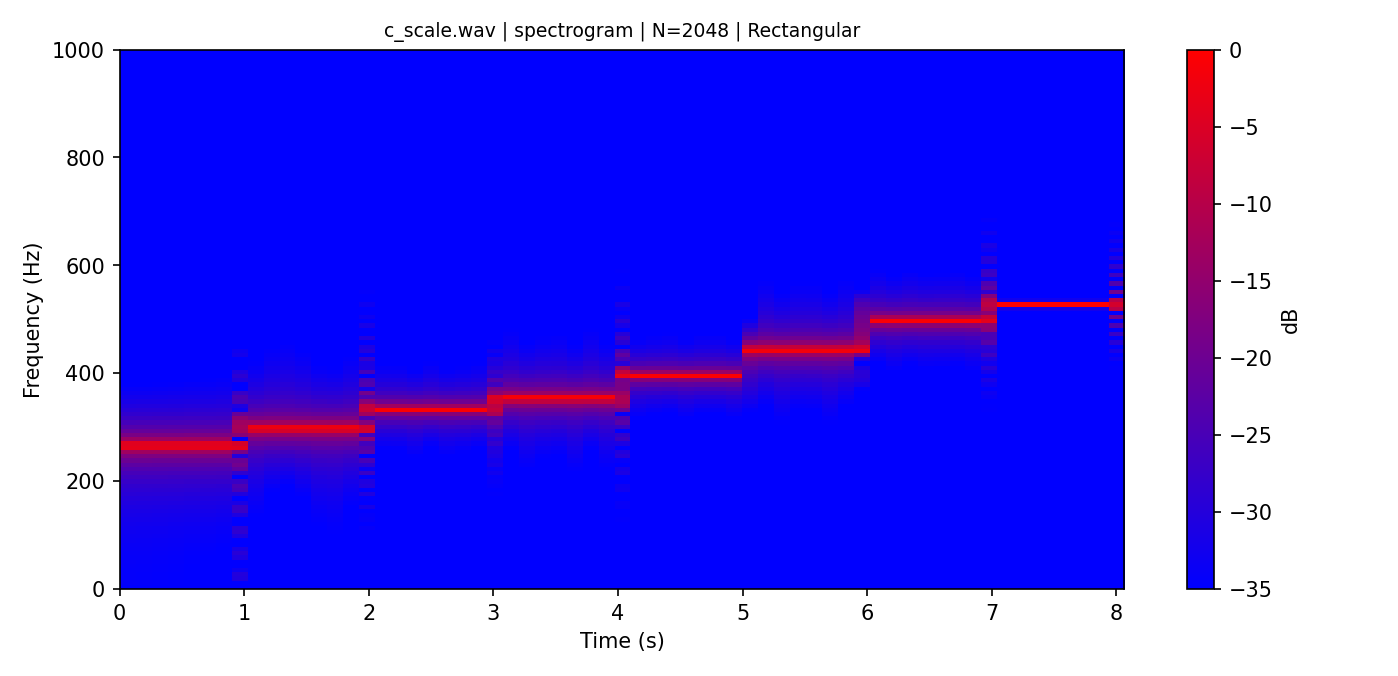
\includegraphics[width=\linewidth]{p1_cscale_N2048.png}
  \caption{Spectrogram of \texttt{c\_scale.wav}, $N = 2048$, Rectangular window, floor $-35$ dB.}
  \label{fig:cscale2048}
\end{figure}

\textbf{What happens where the note changes?} I can see the signal move from one frequency to the next. At each change there is a short overlap where two frequencies appear together. A block that contains the change holds part of the old note and part of the new one, so both frequencies are present in that block. In Figure~\ref{fig:cscale2048} this is the faint vertical smear at each whole second.

\textbf{What does the block size change?} Figure~\ref{fig:cscaleN} shows the same file with a small and a large block.
\begin{itemize}
  \item With the larger block ($N = 8192$) the lines are thin. I can see more clearly which two frequencies are involved in each change, and I am more confident of the frequency of each note. The cost is time. A block lasts 512 ms and is not aligned with the notes, so a change is spread over a whole block.
  \item With the smaller block ($N = 256$) the lines become wide bands. Each bin is 62.5 Hz wide, so neighbouring notes fall in almost the same bins and the change in frequency is hard to tell apart. The time of each change is much sharper.
\end{itemize}

\begin{figure}[H]
  \centering
  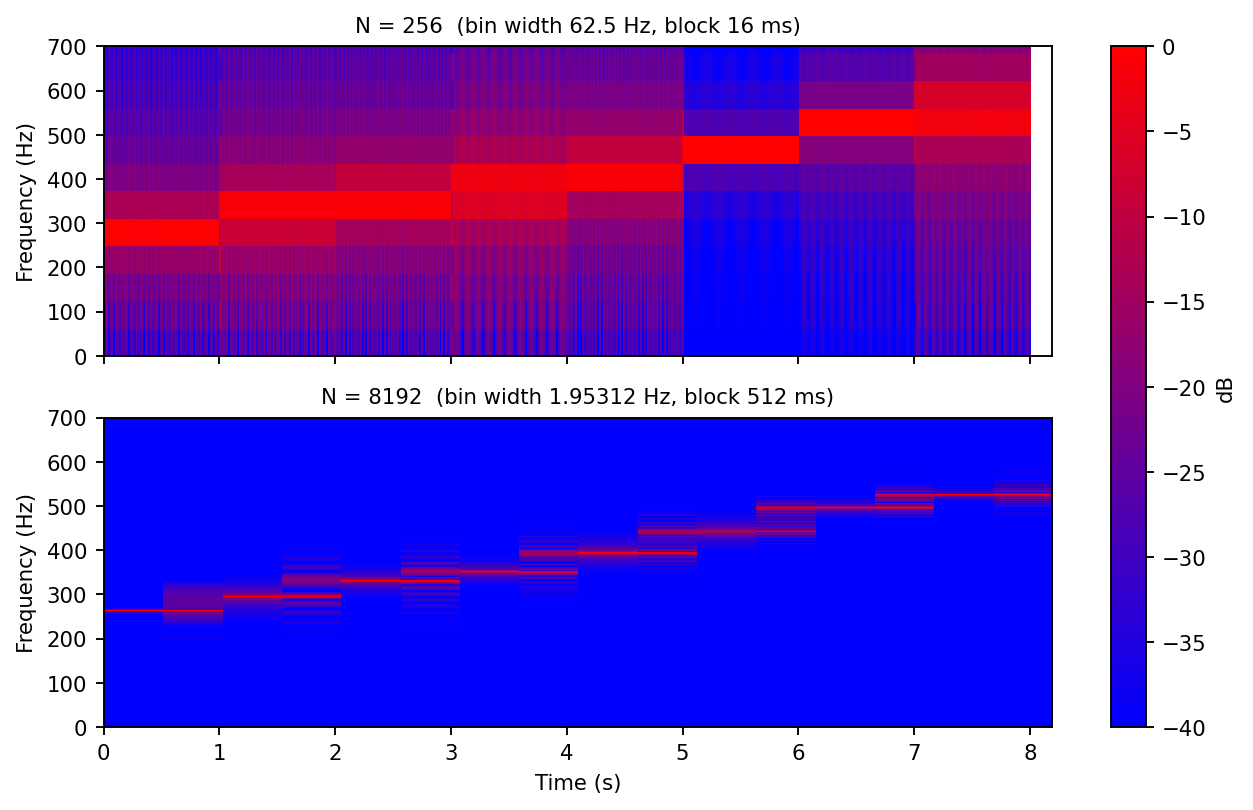
\includegraphics[width=\linewidth]{p1_cscale_N256_N8192.png}
  \caption{Spectrogram of \texttt{c\_scale.wav} with a small and a large block, Rectangular window, floor $-40$ dB.}
  \label{fig:cscaleN}
\end{figure}

\subsection{Block by block, block size and window (step 4)}

I stepped through the scale one block at a time, starting at $N = 2048$. The peak moves from one note to the next between blocks. In the block that contains a change, two peaks appear.

\textbf{Block size.} Figure~\ref{fig:single} shows one block from the third note (330 Hz) for three block sizes. The larger the block, the narrower the peak at its base, and the more certain the frequency. With $N = 256$ the peak is wide and the frequency can only be placed roughly.

\begin{figure}[H]
  \centering
  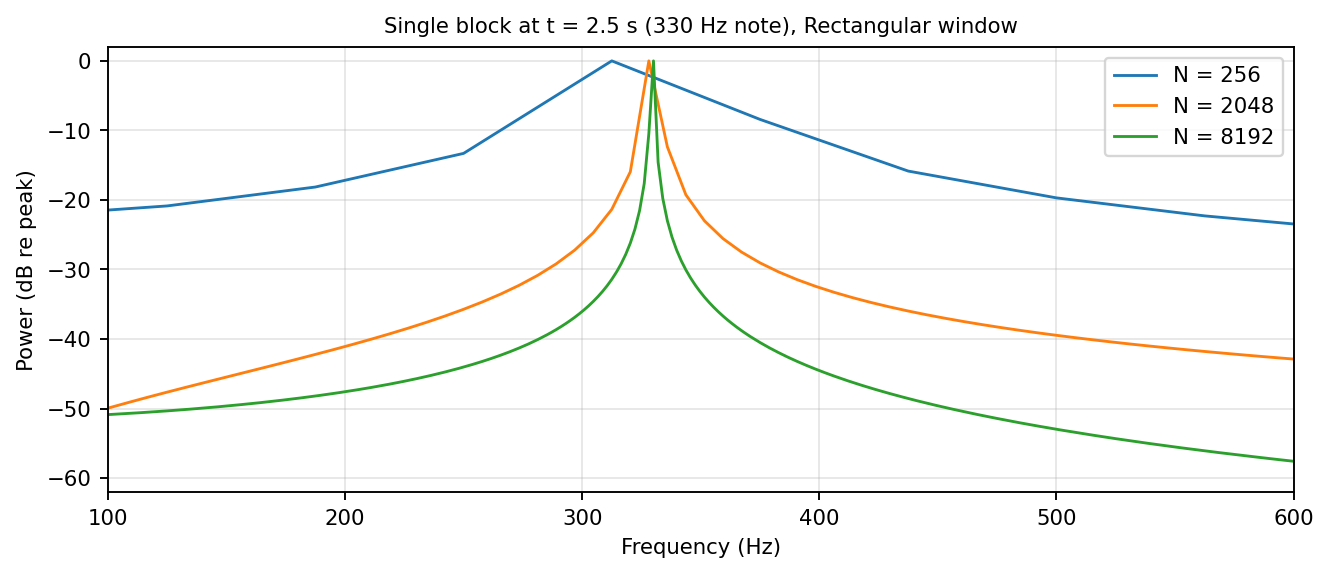
\includegraphics[width=0.9\linewidth]{p1_cscale_single_blocksize.png}
  \caption{One block at $t = 2.5$ s for three block sizes, Rectangular window.}
  \label{fig:single}
\end{figure}

\textbf{Window.} Figure~\ref{fig:windows} compares the three windows at $N = 2048$.
\begin{itemize}
  \item In a steady block (left), 200 Hz away from the peak the Rectangular window is still at about $-41$ dB. Hamming is at about $-59$ dB and Hanning is below $-80$ dB.
  \item In the transition block (right), the peak is the new note (393 Hz). The old note (350 Hz) shows as a shoulder at about $-9$ dB with the Rectangular window and about $-16$ dB and $-17$ dB with Hamming and Hanning. The Rectangular window also adds a ripple. Hamming and Hanning are almost the same here.
\end{itemize}

Whatever the block size or window, the transition blocks show a disturbance as the signal moves from one frequency to the other.

\begin{figure}[H]
  \centering
  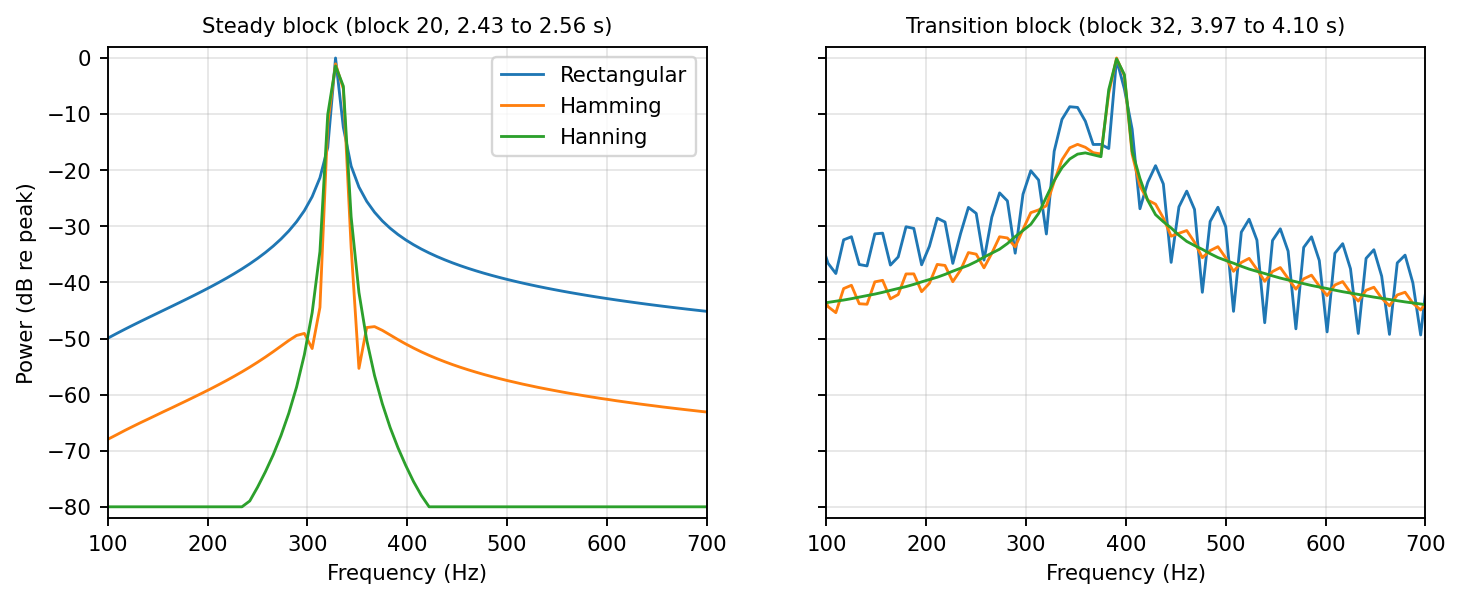
\includegraphics[width=\linewidth]{p1_cscale_windows.png}
  \caption{Single blocks at $N = 2048$ for the three windows. Left: steady block. Right: block that contains the change from 350 Hz to 393 Hz.}
  \label{fig:windows}
\end{figure}

\textbf{Which window do I prefer?} I prefer the Hamming window. It removes the ripple of the Rectangular window and I get a clear view of the transitions. It seems to smooth the signal.

\subsection{Spectrogram of the music (step 5)}

Figures~\ref{fig:m128} and~\ref{fig:m16384} show \texttt{music.wav} (10 s) with the smallest and the largest block I used, over 0 to 2000 Hz.

\begin{figure}[H]
  \centering
  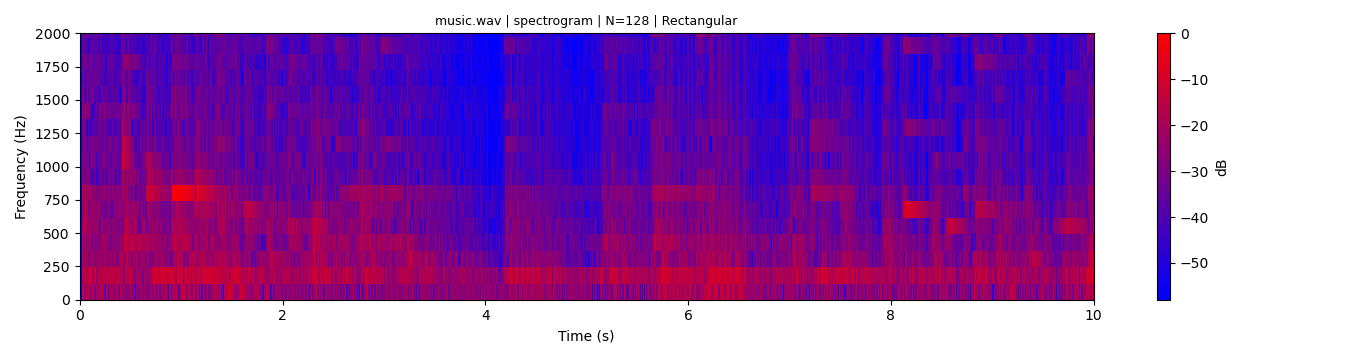
\includegraphics[width=\linewidth]{p1_music_N128.png}
  \caption{Spectrogram of \texttt{music.wav}, $N = 128$ (125 Hz per bin, 8 ms per block), Rectangular window.}
  \label{fig:m128}
\end{figure}

\begin{figure}[H]
  \centering
  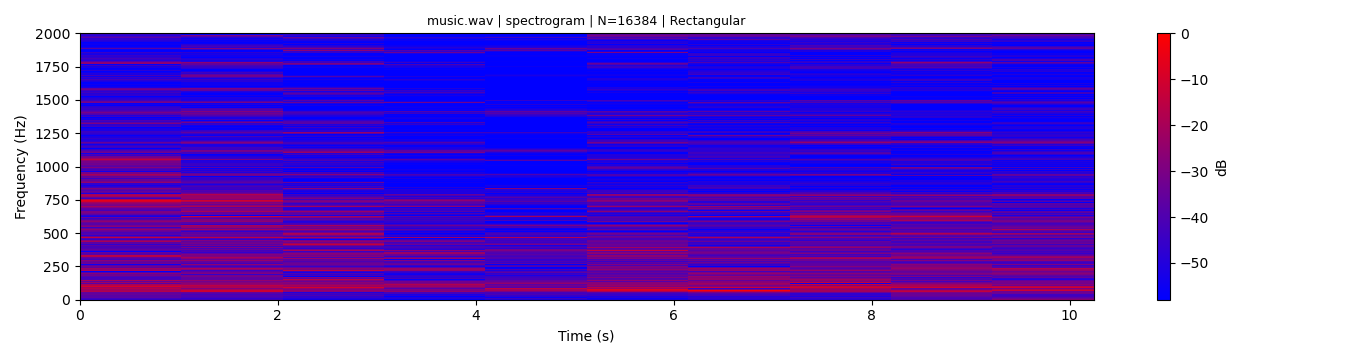
\includegraphics[width=\linewidth]{p1_music_N16384.png}
  \caption{Spectrogram of \texttt{music.wav}, $N = 16384$ (about 1 Hz per bin, 1.02 s per block), Rectangular window.}
  \label{fig:m16384}
\end{figure}

With $N = 16384$ the spectrogram has fine frequency resolution but only one column per second. I see many thin horizontal lines. They are sustained notes and their harmonics, stacked on top of each other. With $N = 128$ the lines merge into broad bands, but events are located sharply in time. For example, the quiet moment near 4 s and the bright patch near 1 s at about 800 Hz are clear. The band near 250 Hz is present throughout.

Most of the energy is at low frequency: 97 \% of the average power is below 3 kHz and 92 \% is below 1 kHz. The quietest part of the clip is around 3 to 5 s (RMS about 0.016 to 0.018, compared with about 0.04 in the first two seconds).

% -------------------------------------------------------
% PART II
% -------------------------------------------------------
\section{Part II: Noise Removal}

\subsection{Audio}

For each file I listened first, then looked at the spectrogram of the noisy file, and then chose a filter. The noise was often not visible at the default floor. I had to lower the floor to about $-80$ dB to see it. Table~\ref{tab:audio} lists the best result I reached for each file. Each filtered \texttt{.wav} file is in the \texttt{Submission} folder, with the filter and its parameters in the file name. Each figure below shows the noisy file above and the filtered file below, with the same settings ($N = 2048$, Hanning window, floor $-80$ dB) and with dB measured from the maximum of the noisy file.

\begin{table}[H]
\centering
\footnotesize
\begin{tabular}{p{4.2cm}p{2.9cm}p{3.7cm}rr}
\toprule
File & Noise & Filter & \multicolumn{2}{c}{SNR (dB)} \\
 & & & before & after \\
\midrule
\texttt{c\_scale\_nb700-2000r8000} & Narrowband & Lowpass 600 Hz & 10.9 & 19.0 \\
\texttt{c\_scale\_p1r5000} & Random, 10 \% of samples & Lowpass 1000 Hz & 24.9 & 33.9 \\
\texttt{c\_scale\_s400r5000} & Sine, 400 Hz & Notch 390 to 410 Hz & 13.2 & 10.4 \\
\texttt{music\_nb400-700r2000} & Narrowband & Notch 400 to 700 Hz & $-2.2$ & 9.0 \\
\texttt{music\_nb5000-7999r3000} & Narrowband & Lowpass 3000 Hz & $-5.7$ & 15.8 \\
\texttt{music\_p01r500} & Random, 1 \% of samples & Median, window 3, threshold 0.01 & 30.0 & 18.2 \\
\texttt{music\_p05r2000} & Random, 5 \% of samples & Median, window 3, threshold 0.001 & 11.0 & 15.0 \\
\texttt{music\_s120r7000} & Sine, 120 Hz & Notch 100 to 200 Hz & $-14.8$ & 10.2 \\
\texttt{music\_s350r5000} & Sine, 350 Hz & Notch 320 to 400 Hz & $-11.9$ & 13.8 \\
\bottomrule
\end{tabular}
\caption{Best result for each noisy audio file. All filters are order 4 where an order applies.}
\label{tab:audio}
\end{table}

\subsubsection*{\texttt{c\_scale\_nb700-2000r8000.wav}}

In the spectrogram I noticed noise above 600 Hz, while the notes of the scale are all below 530 Hz. A lowpass filter with a cutoff of 600 Hz removed it and did the job quite well.

\begin{figure}[H]
  \centering
  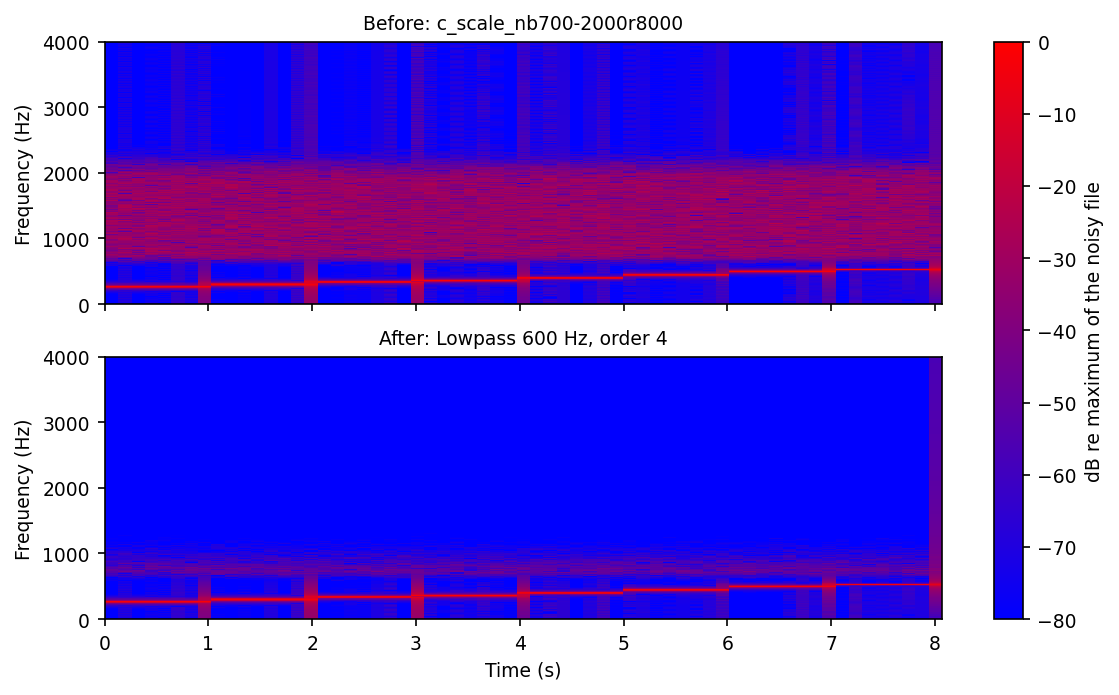
\includegraphics[width=\linewidth]{p2_cscale_nb.png}
  \caption{\texttt{c\_scale\_nb700-2000r8000}: before and after a 600 Hz lowpass.}
\end{figure}

\subsubsection*{\texttt{c\_scale\_p1r5000.wav}}

This one was confusing at first, because at the default floor the spectrogram looked clean. Lowering the floor showed the noise, which is spread over all frequencies. I used a lowpass filter with a cutoff of 1000 Hz. It gave the best result of the two filters I compared: a median filter (window 3, threshold 0) reached 27.7 dB, against 33.9 dB for the lowpass.

\begin{figure}[H]
  \centering
  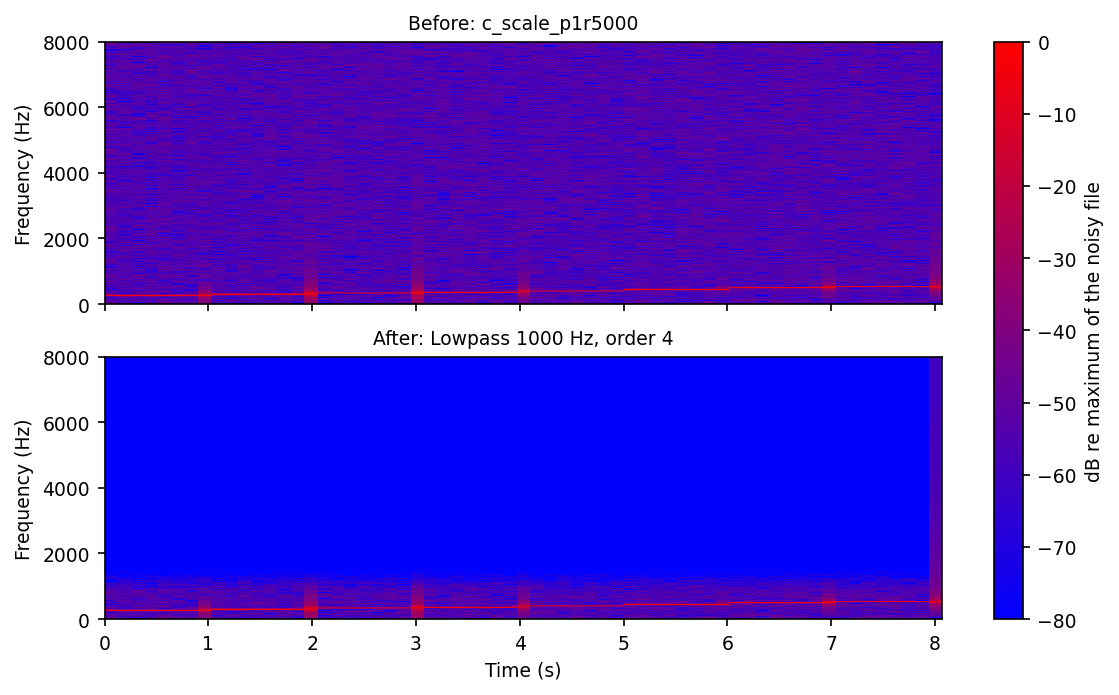
\includegraphics[width=\linewidth]{p2_cscale_p1.png}
  \caption{\texttt{c\_scale\_p1r5000}: before and after a 1000 Hz lowpass.}
\end{figure}

\subsubsection*{\texttt{c\_scale\_s400r5000.wav}}

I applied a notch filter from 390 to 410 Hz. It removed the constant tone around 400 Hz that was in the original file. The fifth note of the scale (393 Hz, from 4 s to 5 s) lies inside this band, so the notch also weakens that note, and the score dropped from 13.2 dB to 10.4 dB. A narrower notch from 399 to 401 Hz scored 34.0 dB in a test, so a narrow band is better here.

\begin{figure}[H]
  \centering
  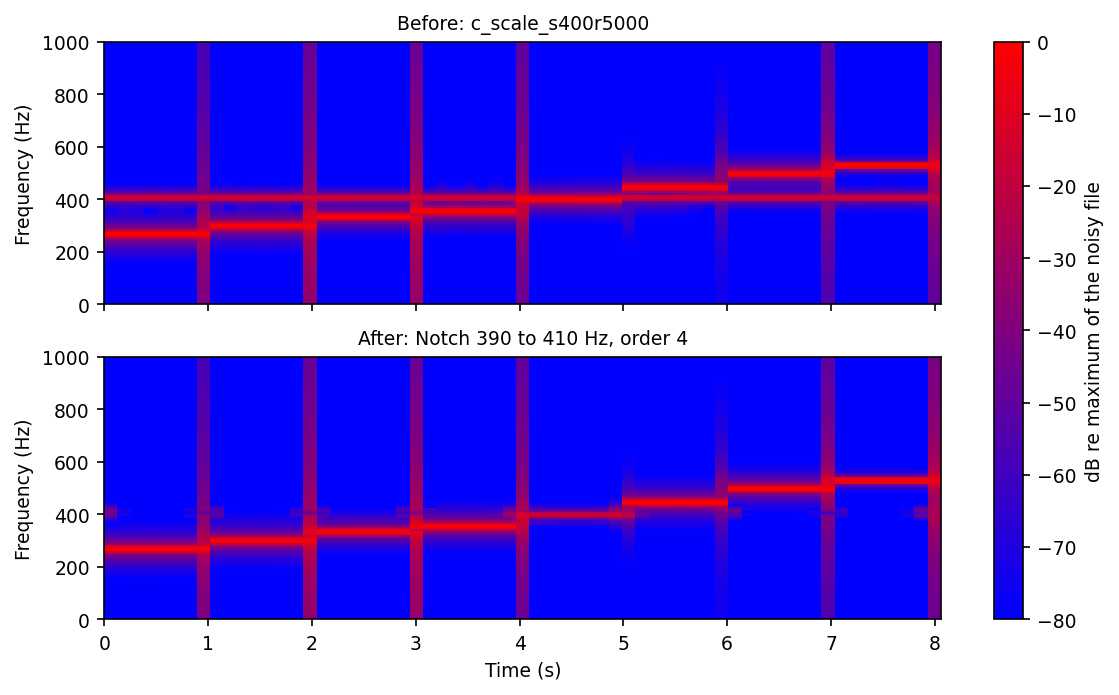
\includegraphics[width=\linewidth]{p2_cscale_s400.png}
  \caption{\texttt{c\_scale\_s400r5000}: before and after a 390 to 410 Hz notch. The 393 Hz note (4 s to 5 s) is also weakened.}
\end{figure}

\subsubsection*{\texttt{music\_nb400-700r2000.wav}}

This was confusing at first because the noise sits in the same range as the music. The spectrogram shows a broad band from 400 to 700 Hz present for the whole file. A notch from 400 to 700 Hz removed it. The music inside that band is removed as well, so the result sounds thinner than the original.

\begin{figure}[H]
  \centering
  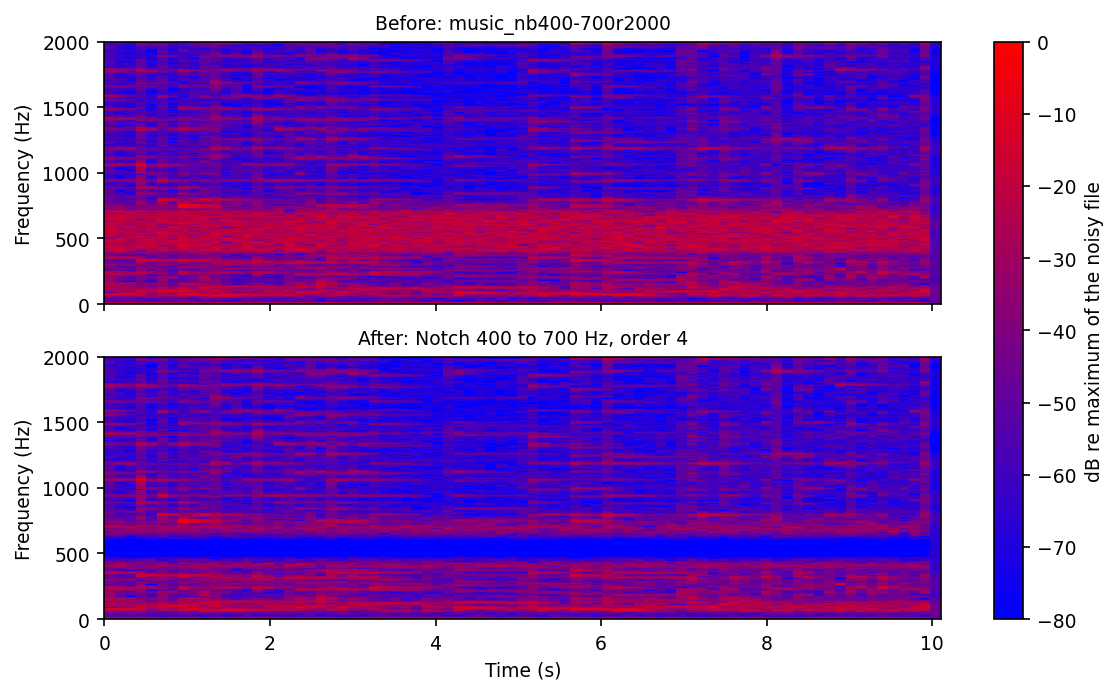
\includegraphics[width=\linewidth]{p2_music_nb400.png}
  \caption{\texttt{music\_nb400-700r2000}: before and after a 400 to 700 Hz notch.}
\end{figure}

\subsubsection*{\texttt{music\_nb5000-7999r3000.wav}}

Here the noise band is well above the music, so I applied a lowpass filter with a cutoff of 3000 Hz.

\begin{figure}[H]
  \centering
  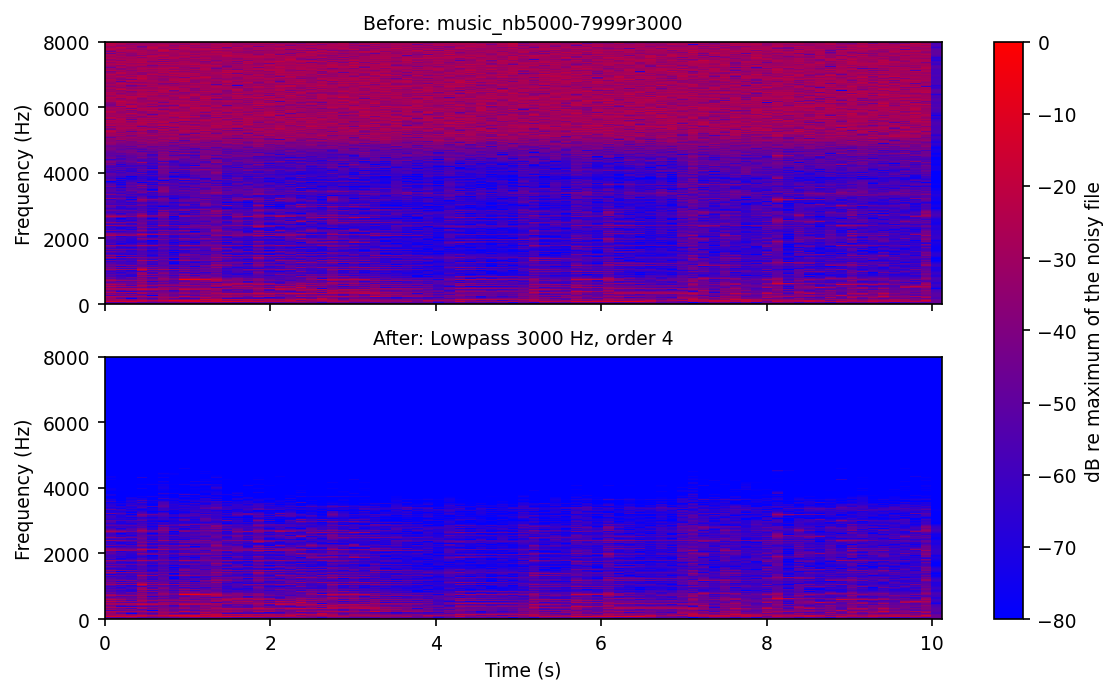
\includegraphics[width=\linewidth]{p2_music_nb5000.png}
  \caption{\texttt{music\_nb5000-7999r3000}: before and after a 3000 Hz lowpass.}
\end{figure}

\subsubsection*{\texttt{music\_p01r500.wav}}

I used a median filter with window 3 and threshold 0.01. I could still hear some tiny noises afterwards. The score shows that the filter did not help: it fell from 30.0 dB to 18.2 dB. This file is already close to clean, and its noise (at most 0.015) is smaller than the natural change from sample to sample in the music. The filter cannot tell the two apart and replaces some real samples. For this file I would leave the original as it is.

\begin{figure}[H]
  \centering
  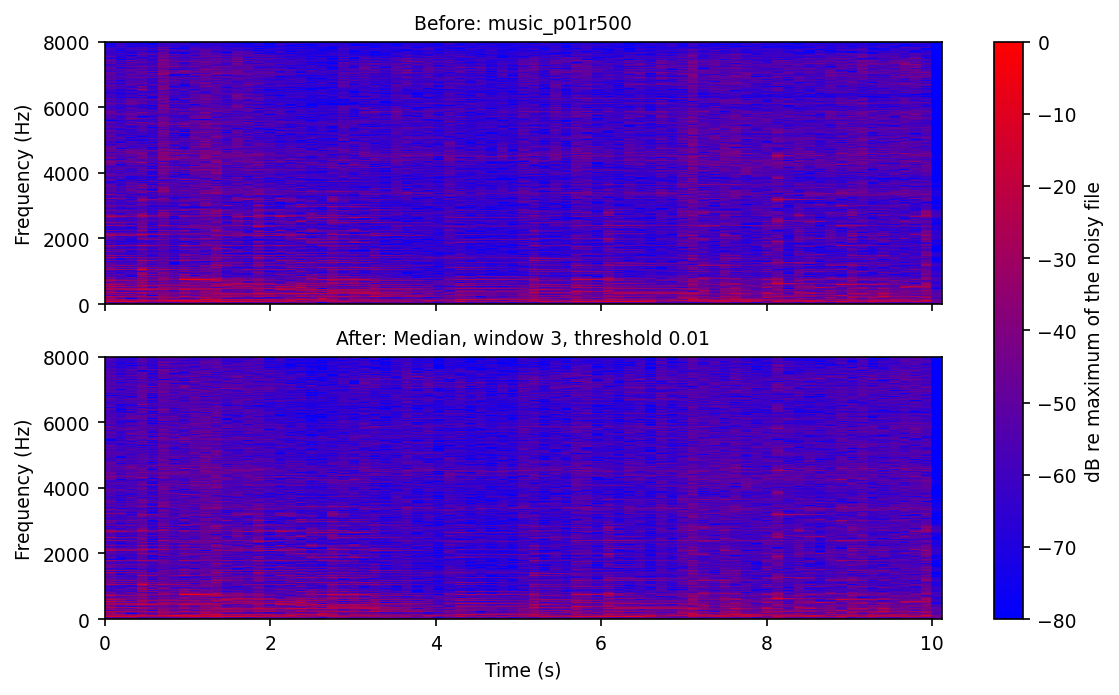
\includegraphics[width=\linewidth]{p2_music_p01.png}
  \caption{\texttt{music\_p01r500}: before and after a median filter (window 3, threshold 0.01).}
\end{figure}

\subsubsection*{\texttt{music\_p05r2000.wav}}

I was very disturbed by this one at first, because the median filter seemed not to work. After trying different windows and thresholds, a window of 3 and a threshold of 0.001 worked best. I can still hear a slight perturbation in the sound, but this was the closest I could get. A window of 7 with the same threshold scored only 11.7 dB, against 15.0 dB for a window of 3.

\begin{figure}[H]
  \centering
  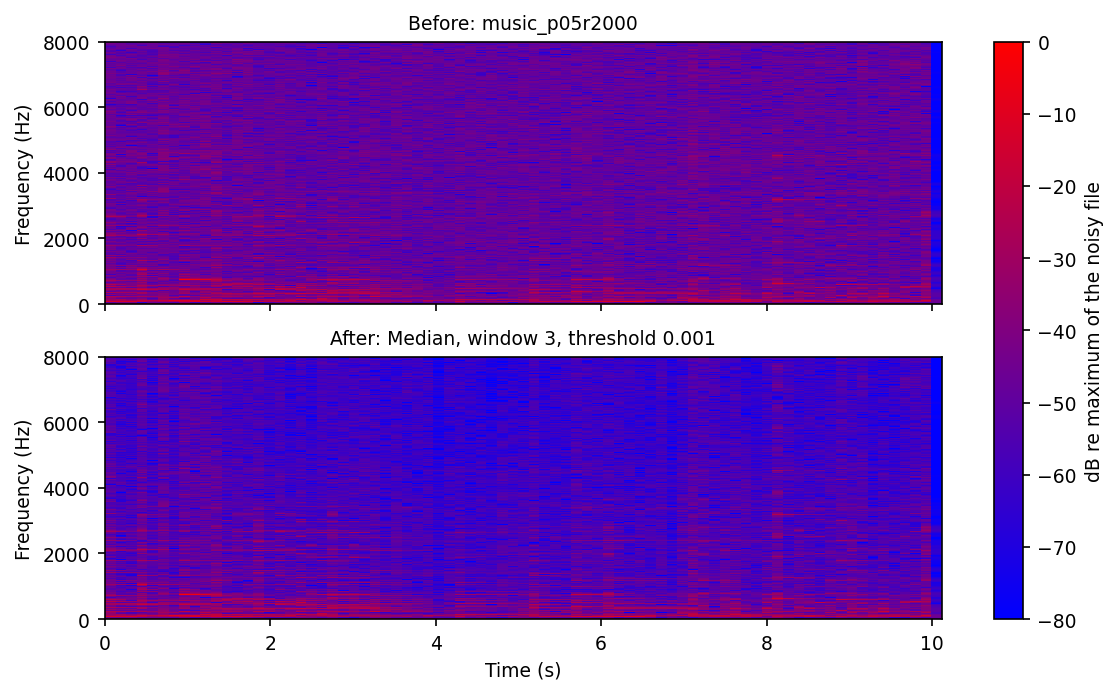
\includegraphics[width=\linewidth]{p2_music_p05.png}
  \caption{\texttt{music\_p05r2000}: before and after a median filter (window 3, threshold 0.001).}
\end{figure}

\subsubsection*{\texttt{music\_s120r7000.wav} and \texttt{music\_s350r5000.wav}}

For both files the noise was clear the moment I played them: a constant tone. In the spectrogram it sits at one frequency. For \texttt{music\_s120r7000} I used a notch from 100 to 200 Hz, and for \texttt{music\_s350r5000} a notch from 320 to 400 Hz. Both removed the tone. The bands are wider than the tones (120 Hz and 350 Hz), so some of the music inside them is removed as well.

\begin{figure}[H]
  \centering
  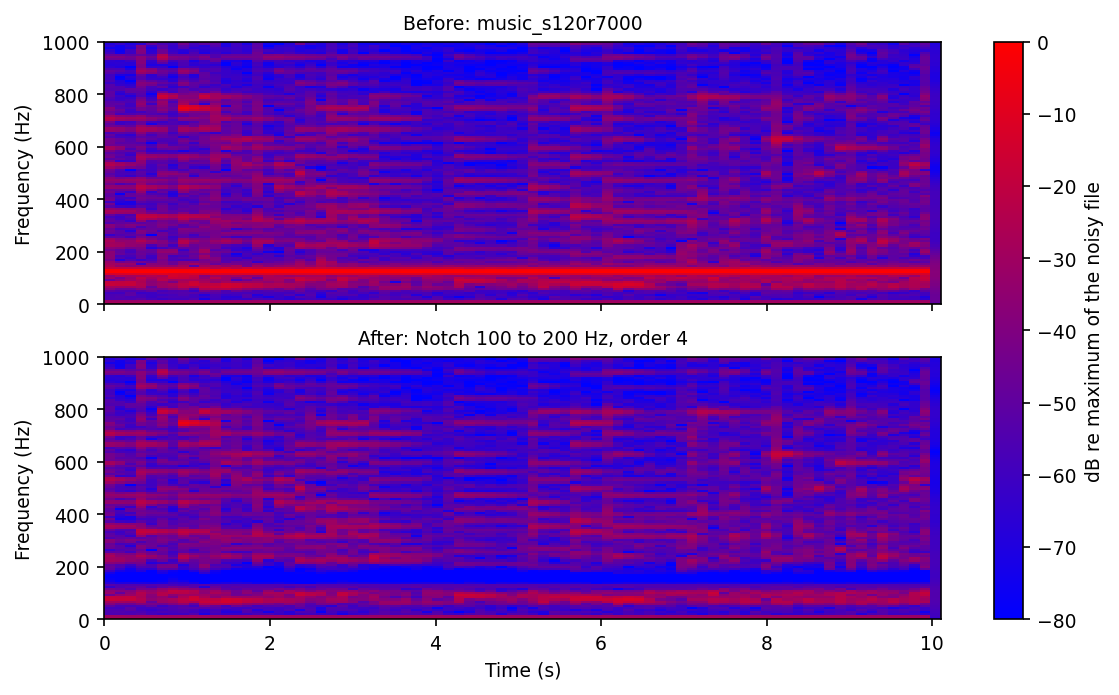
\includegraphics[width=\linewidth]{p2_music_s120.png}
  \caption{\texttt{music\_s120r7000}: before and after a 100 to 200 Hz notch.}
\end{figure}

\begin{figure}[H]
  \centering
  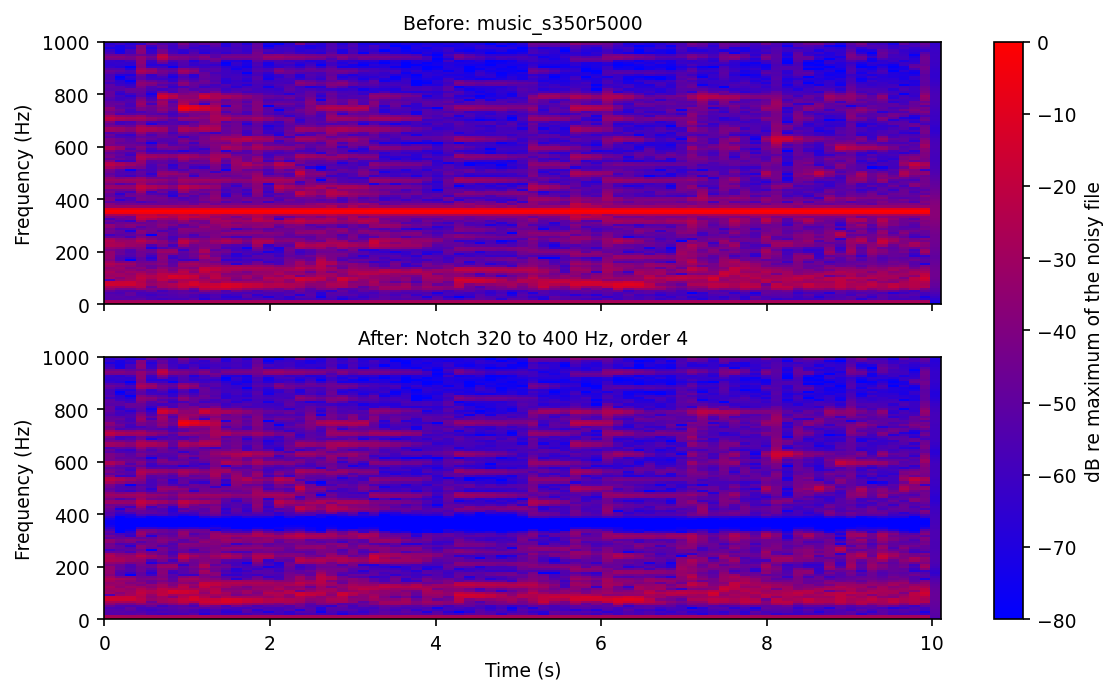
\includegraphics[width=\linewidth]{p2_music_s350.png}
  \caption{\texttt{music\_s350r5000}: before and after a 320 to 400 Hz notch.}
\end{figure}

\subsection{Images}

The four noisy images contain random noise on a small part of the pixels, up to about 10 \% for the \texttt{p1} files and 5 \% for the \texttt{p05} files, in each colour channel. The noise appears as single coloured dots (Figure~\ref{fig:photo}). I compared a median filter (window 3 and 5) and a Gaussian filter (sigma 1 and 2).

\textbf{Median filter.} A median filter with a window of 3 removed the noise from all four images, so it is my best result for each of them. Figure~\ref{fig:median3} shows the four outputs and Table~\ref{tab:img} gives the scores of all the filters I compared.

\begin{figure}[H]
  \centering
  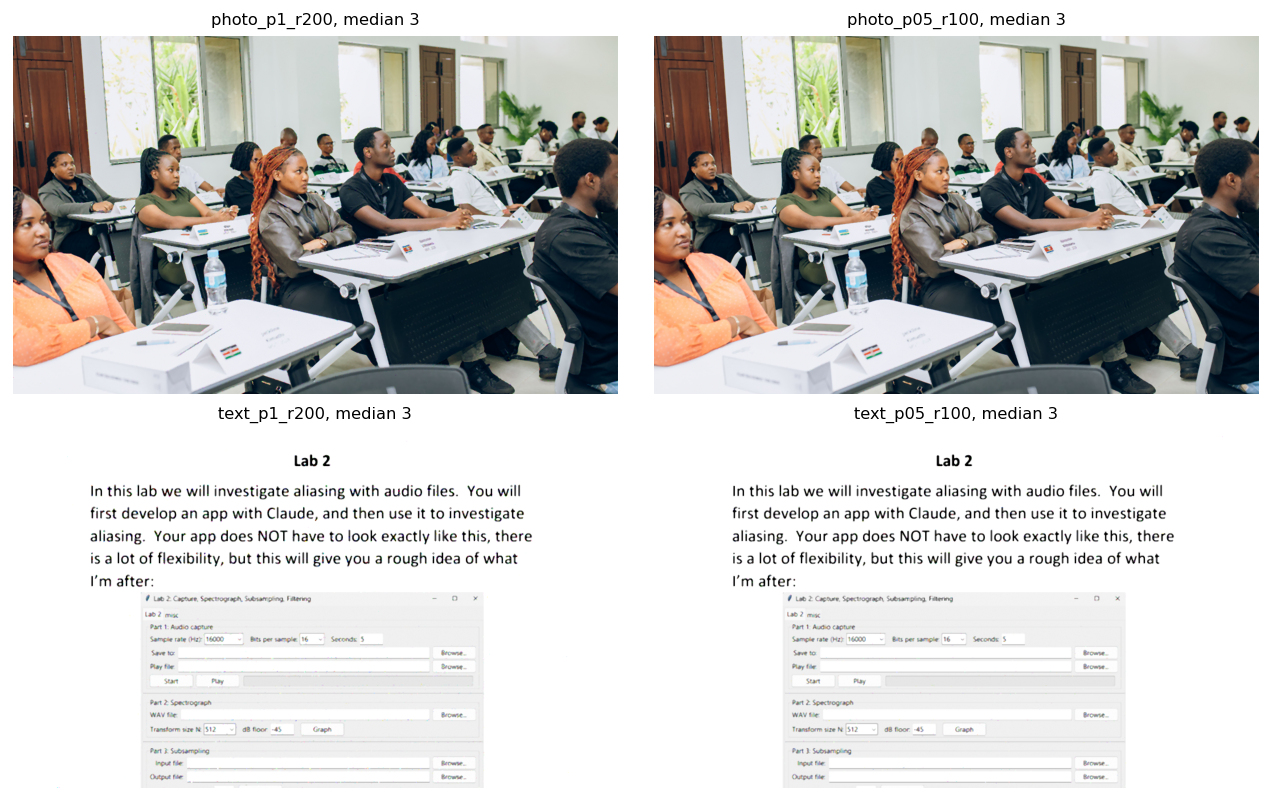
\includegraphics[width=\linewidth]{p2_img_median3_all.png}
  \caption{Median filter, window 3, applied to the four noisy images.}
  \label{fig:median3}
\end{figure}

The noise is removed at the cost of the finer details. In the photograph, the skin texture and the braids are softer. In the text, the thin strokes of the letters are thinner and the edges are less sharp (Figures~\ref{fig:photo} and~\ref{fig:text}).

\textbf{Gaussian filter.} The Gaussian filter was very sensitive to sigma and was not able to handle this noise. A Gaussian blur does not remove a noisy pixel. It spreads it into its neighbours, so faint speckle remains while the image already looks blurred. A larger sigma only blurs more.

\textbf{Larger median window.} The same applies to the median filter. A window of 5 removes the noise but damages the picture more, and the text letters start to break up.

\begin{figure}[H]
  \centering
  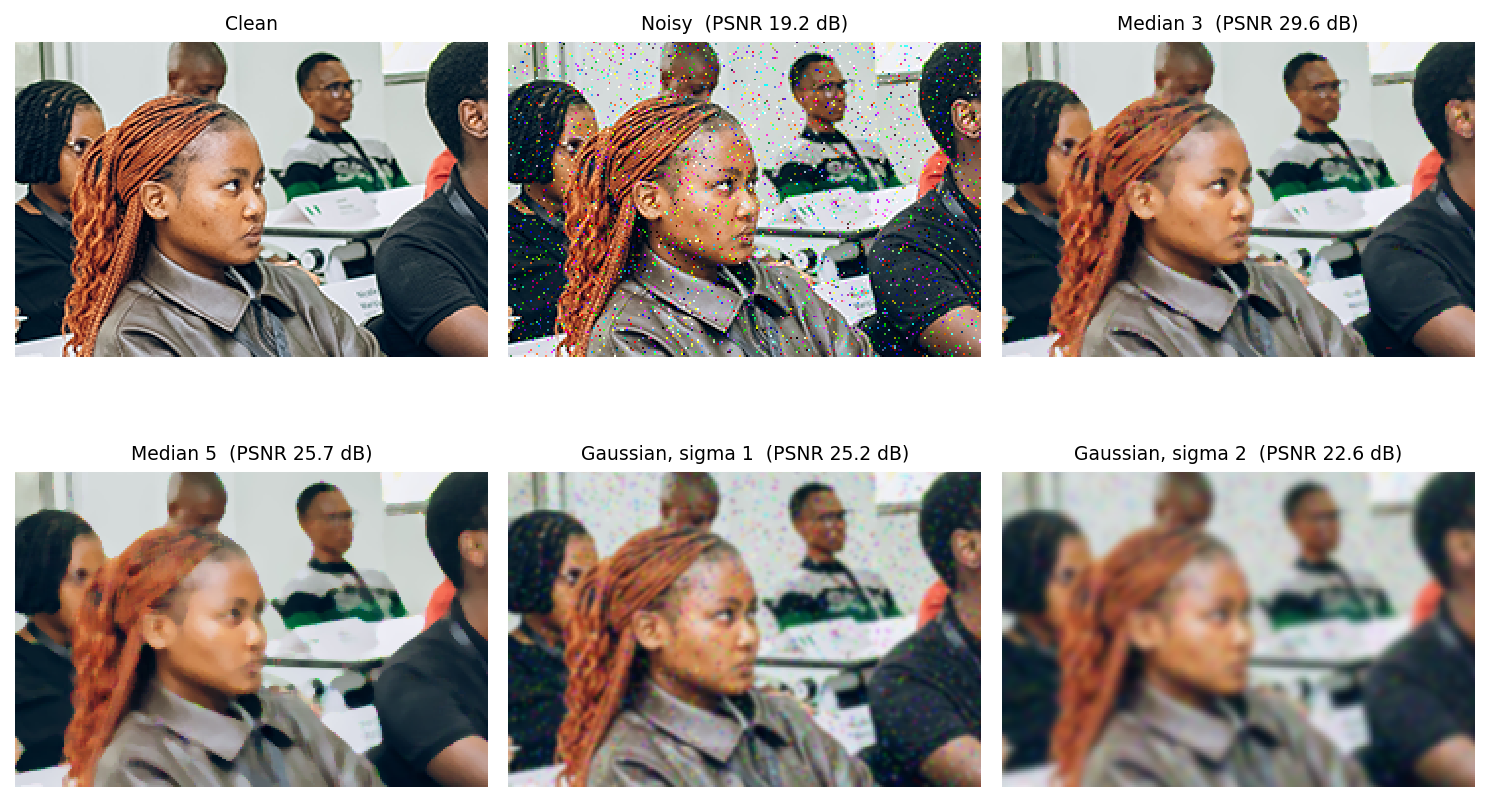
\includegraphics[width=\linewidth]{p2_img_photo_compare.png}
  \caption{Part of \texttt{photo\_p1\_r200} for the clean image, the noisy image and four filters. The PSNR is for the whole image.}
  \label{fig:photo}
\end{figure}

\begin{figure}[H]
  \centering
  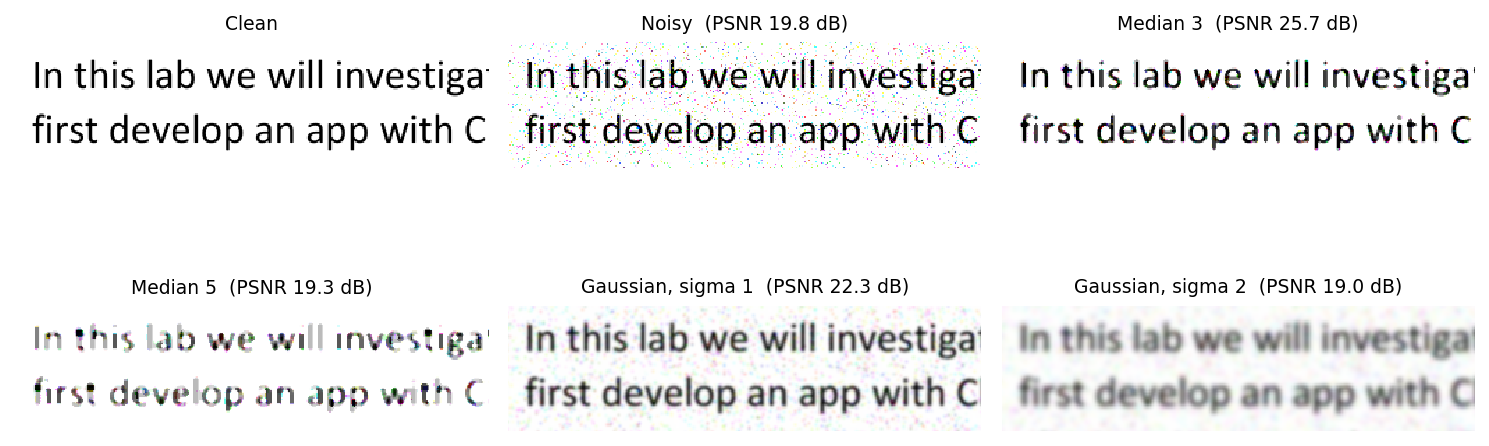
\includegraphics[width=\linewidth]{p2_img_text_compare.png}
  \caption{Part of \texttt{text\_p1\_r200} for the clean image, the noisy image and four filters. The PSNR is for the whole image.}
  \label{fig:text}
\end{figure}

\begin{table}[H]
\centering
\footnotesize
\begin{tabular}{lrrrrr}
\toprule
File & Noisy & Median 3 & Median 5 & Gaussian, $\sigma=1$ & Gaussian, $\sigma=2$ \\
\midrule
\texttt{photo\_p1\_r200}  & 19.2 & \textbf{29.6} & 25.7 & 25.2 & 22.6 \\
\texttt{photo\_p05\_r100} & 27.3 & \textbf{30.4} & 25.9 & 27.1 & 23.0 \\
\texttt{text\_p1\_r200}   & 19.8 & \textbf{25.7} & 19.3 & 22.3 & 19.0 \\
\texttt{text\_p05\_r100}  & \textbf{28.7} & 26.0 & 19.2 & 23.3 & 19.2 \\
\bottomrule
\end{tabular}
\caption{PSNR (dB) against the clean image. The best value in each row is in bold.}
\label{tab:img}
\end{table}

\textbf{Photograph and text.} The two image types react differently.
\begin{itemize}
  \item The photograph tolerates filtering better. It has smooth areas, and the median filter lifts the score a lot (19.2 dB to 29.6 dB for \texttt{p1}).
  \item The text is made of thin, high-contrast strokes, so any filter that mixes neighbouring pixels damages it sooner. The gain from the median filter is smaller, and a window of 5 is already worse than the noisy image for \texttt{p1} (19.3 dB against 19.8 dB).
  \item For the lightly noised text, \texttt{text\_p05\_r100}, the median filter removes the dots but scores lower than the noisy image (26.0 dB against 28.7 dB). The damage to the strokes is larger than the damage from the few noisy pixels. The score is only a guide here, because visually the dots are gone.
\end{itemize}

% -------------------------------------------------------
% SUMMARY
% -------------------------------------------------------
\section{Summary}

\begin{itemize}
  \item The spectrum shows where the noise is, so look at it before choosing a filter. Lower the floor to see weak noise.
  \item A notch removes a tone or a band. A lowpass removes noise that sits above the music. Both also remove any music in the same frequencies, so the band should be as narrow as the noise allows.
  \item A median filter suits random noise on a few samples, but only when the noise is larger than the natural change in the signal.
  \item For images, the median filter with a small window worked best. Larger windows and Gaussian blur remove detail without removing the noise.
\end{itemize}

% -------------------------------------------------------
% FILES
% -------------------------------------------------------
\section{Files}

The Lab 3 folder contains the following.
\begin{itemize}
  \item The application source code and its tests, with a \texttt{README.md} that lists every file.
  \item \texttt{data/}: the lab input files.
  \item \texttt{Submission/}: the filtered audio and image files and the figures saved from the application.
  \item \texttt{latex/}: the source of this report and its figures in \texttt{images/}. The additional figures were generated with \texttt{scripts/make\_report\_figures.py}.
\end{itemize}

\end{document}
